\documentclass[a4paper,12pt,titlepage]{article}
\usepackage[utf8]{inputenc}
\usepackage{textcomp}
\usepackage{geometry}
\usepackage{fancyhdr}
\usepackage{tabularx}
\usepackage{parskip} 
\usepackage{longtable}
\usepackage{graphicx}
\usepackage{booktabs}
\pagestyle{fancy}
\lhead{Malcolm Vigren}
\rhead{D3.c}
\geometry{margin=3cm}

\begin{document}
\section*{Koncept för Snowslide Car Edition}

Snowslide Car Edition är en underhållningstjänst tänkt att ta plats i bilar.
Pia identifieras som den primära personan, och Tom som den sekundära.

\subsection*{Radikala koncept}

3 radikala koncept utvecklades i detta designuppdrag.

\subsubsection*{Koncept 1: Snowslide4U}
Med Snowslide4U kan varje användare till underhållningssystemet ställa in sina
egna profiler för sin underhållning. Exempelvis kan en användare spara sina
favoritfilmer eller serier så att de blir lättåtkomliga, skapa egna
spellistor för musikspelaren, spara favoritrestauranger eller andra platser,
eller organisera de appar som de själva önskar.

Snowslide4U möjliggör även att barn kan ha kul i bilen samtidigt som föräldrarna
har kontroll över det innehåll och mängden barnen konsumerar.
Föräldrar skapar helt enkelt profiler för sina barn,
där exempelvis parametrar baserad på bland annat åldersbegränsning kan ställas in
för vilken media ska kunna tillåtas för vilka profiler, huruvida köp inuti
appar och i medie-affären ska vara tillåtna, samt en maximal visningstid för
filmer eller speltid för spel per dag.

Profilerna kan vid uppstart av systemet tilldelas till vissa säten i bilen.
Detta kan enkelt justeras i gränssnittet genom att varje persons profil syns som
ett ansikte som man kan dra runt i bilen för att tilldelas vissa säten.
Användare av barnprofilerna kan inte justera sina positioner i bilen, så att de inte helt
enkelt kan använda föräldrarnas profiler.

Pias mål som konceptet bidrar till:
\begin{itemize}
    \item Bekvämlighet
    \item När hon reser med barnen vill
        hon att de (åtminstone Tom) ska vara
        sysselsatta så att resan blir lugn.
    \item Vill att Tom ska göra annat än att
        bara titta på teve eller spela datorspel.
    \item Vill inte att Tom ska titta på saker
        på teve eller nätet, eller spela spel,
        som inte är lämpliga för en nioåring.
    \item Vill spara tid. Vill själv hitta
        information snabbt och effektivt: Vill
        inte bläddra igenom oorganiserade
        böcker bara för att hitta en restaurang
        som är öppen sent.
\end{itemize}

Toms mål som konceptet bidrar till:
\begin{itemize}
    \item Hålla sig sysselsatt (alltså inte ha
        tråkigt): Göra det han måste för
        föräldrarna och skolan, men bli klar så
        fort som möjligt. Kolla sina
        favoritfilmer och teveserier, och chatta
        eller söka information om dem på
        nätet. Hitta riktigt roliga, men gratis,
        spel på nätet, så att han kan få nya
        upplevelser utan att behöva be om
        pengar för att köpa saker. 
    \item Vill kolla på sina favoritserier när
        han vill. Eller får för mamma och
        pappa.
\end{itemize}

Målgrupper: Regelbundna användare och föräldrar med barn.

Inga negativa konsekvenser kunde identifieras för detta koncept, som inte rör
all bilunderhållning.

Exempel på storyboard:

\begin{center}
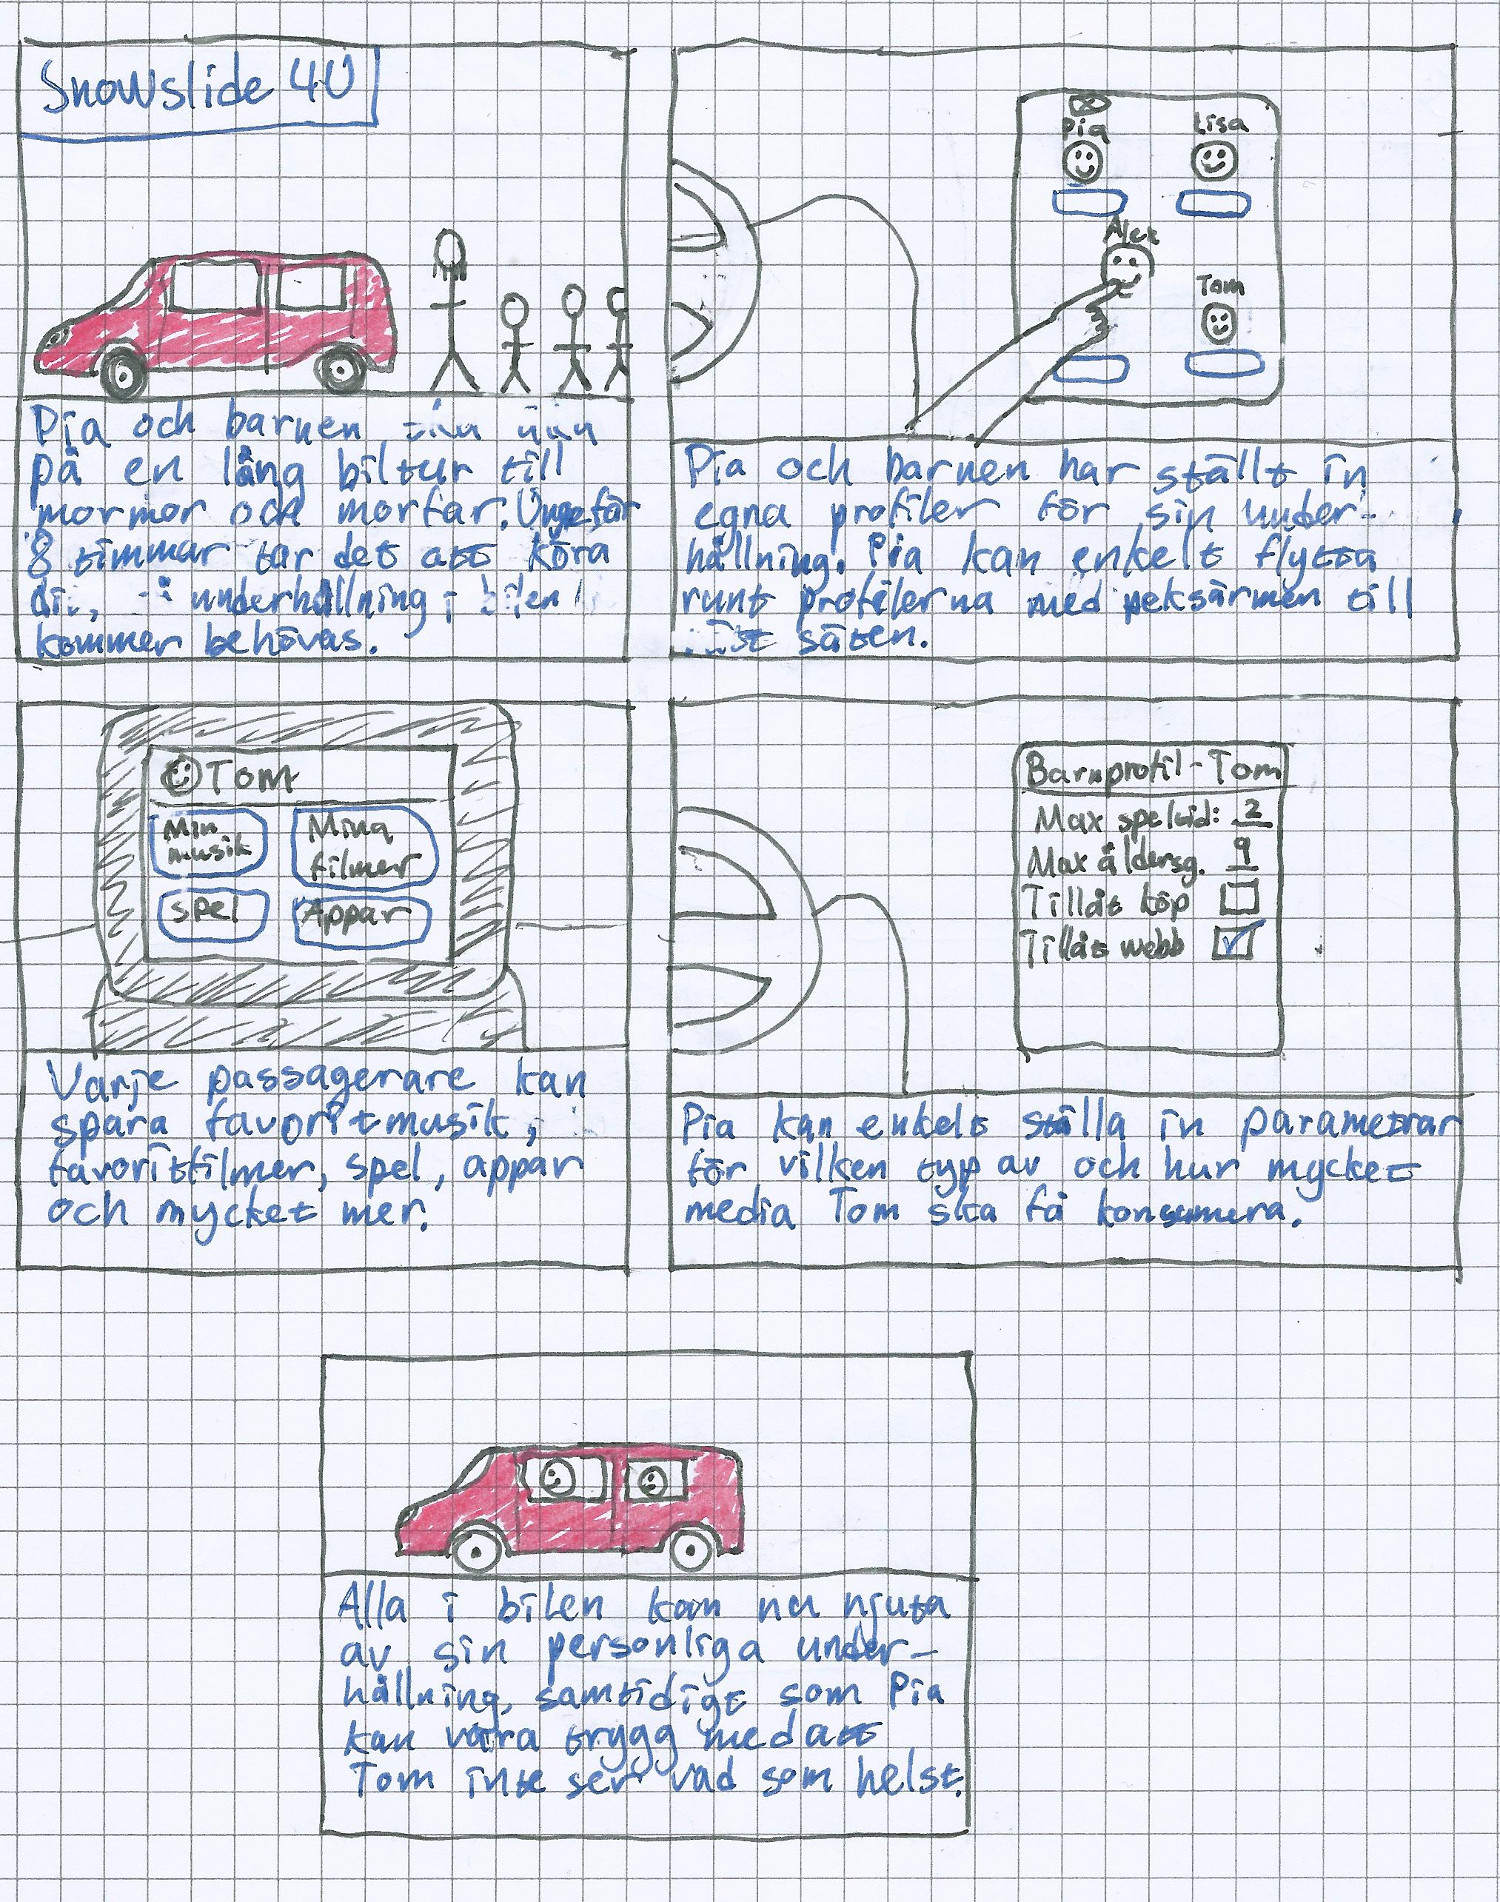
\includegraphics[width=14cm]{images/4u.jpg}
\end{center}

\newpage
\subsubsection*{Koncept 2: Snowslide Connected}

Med Snowslide Connected begränsas inte medieupplevelsen till den bilen man
färdas i. Snowslide Connected gör nämligen att du kan integrera appar med andra
bilar med samma system. Med inkluderade applikationer och verktyg för
tredjepartsutvecklare som använder bilens GPS kan t ex flera bilar spela 
ett "på-spåret"-liknande
frågesport med andra bilar, där bilarna visas på en karta och användarna ska
försöka gissa vart andra användare är på väg, baserat på wikipedia-information
om platsen de ska till. En annan app skulle kunna vara att körningen analyseras
ur ett eco-driving-perspektiv och visar i realtid en lista av vilka som kör
mest miljövänligt i sin stad eller sitt land just nu. Vid sökning av
restauranger eller andra platser skulle information om hur många bilar med
Snowslide som besökt platsen den dagen, tillsammans med recensioner och
användarrapporterad information om någonting är speciellt med stället den
dagen.

Pias mål som konceptet bidrar till:
\begin{itemize}
    \item Bekvämlighet
    \item När hon reser med barnen vill
        hon att de (åtminstone Tom) ska vara
        sysselsatta så att resan blir lugn.
    \item Vill att Tom ska göra annat än att
        bara titta på teve eller spela datorspel.
    \item Vill gärna imponera på kunder.
    \item Söker ibland bara förströelse.
\end{itemize}

Toms mål som konceptet bidrar till:
\begin{itemize}
    \item Hålla sig sysselsatt (alltså inte ha
        tråkigt): Göra det han måste för
        föräldrarna och skolan, men bli klar så
        fort som möjligt. Kolla sina
        favoritfilmer och teveserier, och chatta
        eller söka information om dem på
        nätet. Hitta riktigt roliga, men gratis,
        spel på nätet, så att han kan få nya
        upplevelser utan att behöva be om
        pengar för att köpa saker. 
    \item Ha koola grejer och göra koola
        saker: Ta reda på var man billigast kan
        köpa en Playstation 4 så att mamma
        kanske köper en till nästa födelsedag.
        Hans dröm vore att åka till Legoland i
        Danmark eller Disneyland i Paris
        nästa sommar.
\end{itemize}

Målgrupper: Personer som gillar att interagera med andra människor och folk som
vill ha kul i bilen.

En konsekvens av detta koncept kan vara att användarens integritet inskränks,
om t ex bilens kameror eller GPS-position delas med folk som inte har med den
informationen att göra. Vid realisering av detta koncept bör därför
implementera någon form av samtyckeskontroll med användaren, samt utförlig
säkerhet för att se till att informationen inte kan stjälas av hackare.

\newpage
Exempel på storyboard:

\begin{center}
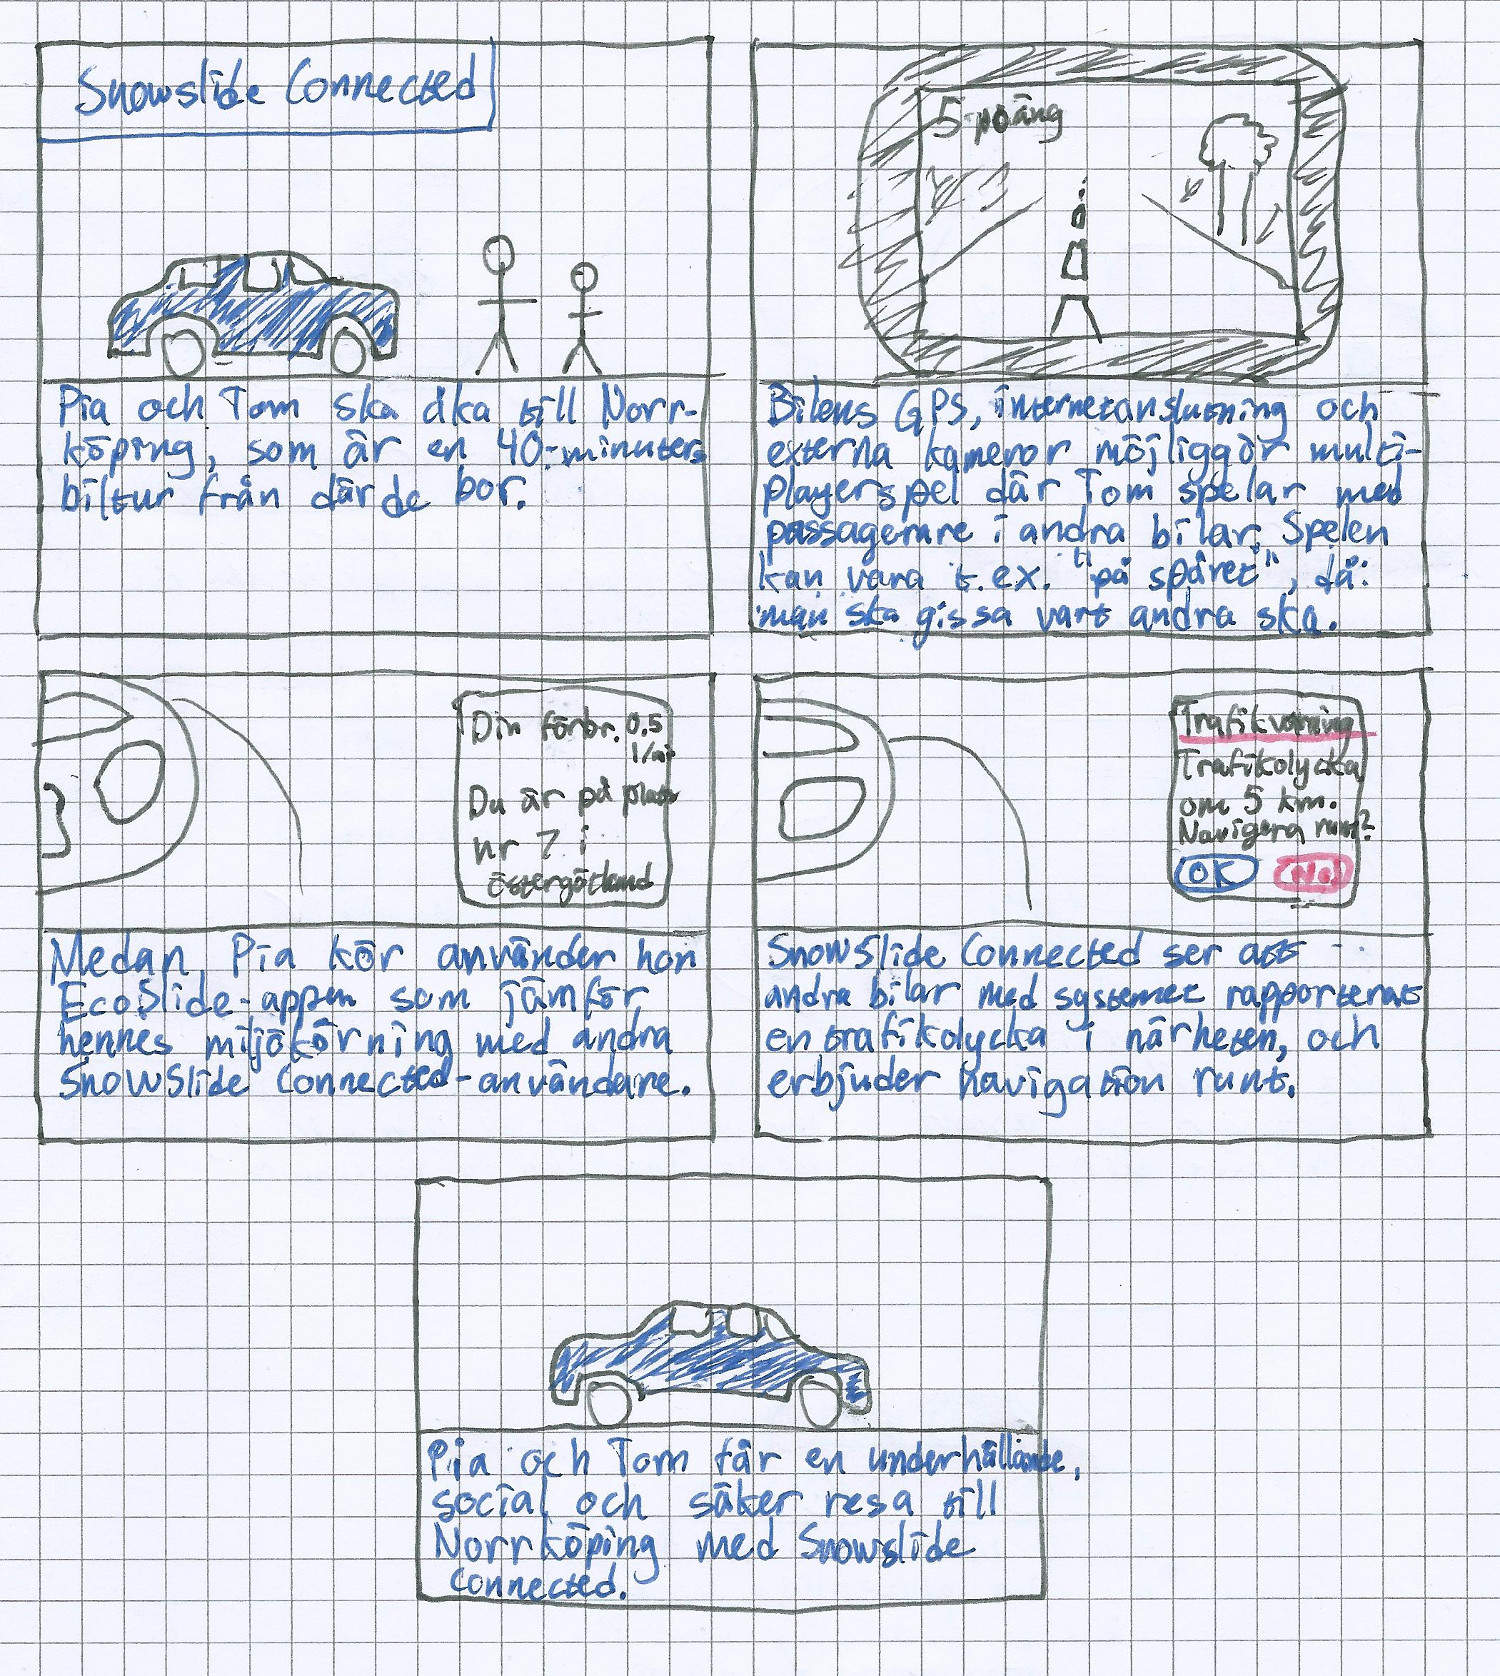
\includegraphics[width=15cm]{images/connected.jpg}
\end{center}

\newpage
\subsubsection*{Koncept 3: Snowslide Assistant}

Att interagera med funktionerna med ett underhållningssystem i bilen som förare
kan vara farligt. Samtidigt kan det kännas onödigt att behöva stanna bilen på
motorvägen bara för att välja en ny spellista i Spotify, eller knappa in en ny
destination på GPS:en.

Med Snowslide Assistant kan man helt och hållet interagera med Snowslide Car
Edition utan att behöva titta bort från vägen. Med en knapp på ratten aktiveras
en röstassistent, med vilken man kan styra alla systemets funktioner.
Exempelvis kan man fråga ``Var finns närmaste bensinmack?'', och systemet kan då
starta en navigation. Man kan också exempelvis be systemet spela en viss spellista i Spotify,
spela upp en viss podcast eller mer komplicerade förfrågningar, som ``Boka bord
hos en italiensk restaurang med bra recensioner, och navigera mig dit''.

Pias mål som konceptet bidrar till:
\begin{itemize}
    \item Bekvämlighet
    \item Vill gärna imponera på kunder.
    \item Vill spara tid. Vill själv hitta
        information snabbt och effektivt: Vill
        inte bläddra igenom oorganiserade
        böcker bara för att hitta en restaurang
        som är öppen sent.
    \item Det vore bra att ha en del
        information om möjliga restauranger
        och nöjen i ett specifikt geografiskt
        område (t.ex.\ runt hotellet, eller i
        närheten av ett stopp) i händelse av
        att hon får tid över innan eller efter
        sina möten. 
\end{itemize}

Målgrupper: Förare och passagerare som inte kan interagera med skärmar men ändå
vill kunna få den information de vill ha.

En möjlig konsekvens av detta är att man kanske tänker för mycket på att få
röstassistenten att förstå vad man säger, vilket kan göra att man blir
distraherad från körningen. Vid realiseringen bör man därför se till att
röstigenkänningstekniken som används är så bra som möjligt, vilket minskar
risken för frustration hos föraren.

\newpage
Exempel på storyboard:

\begin{center}
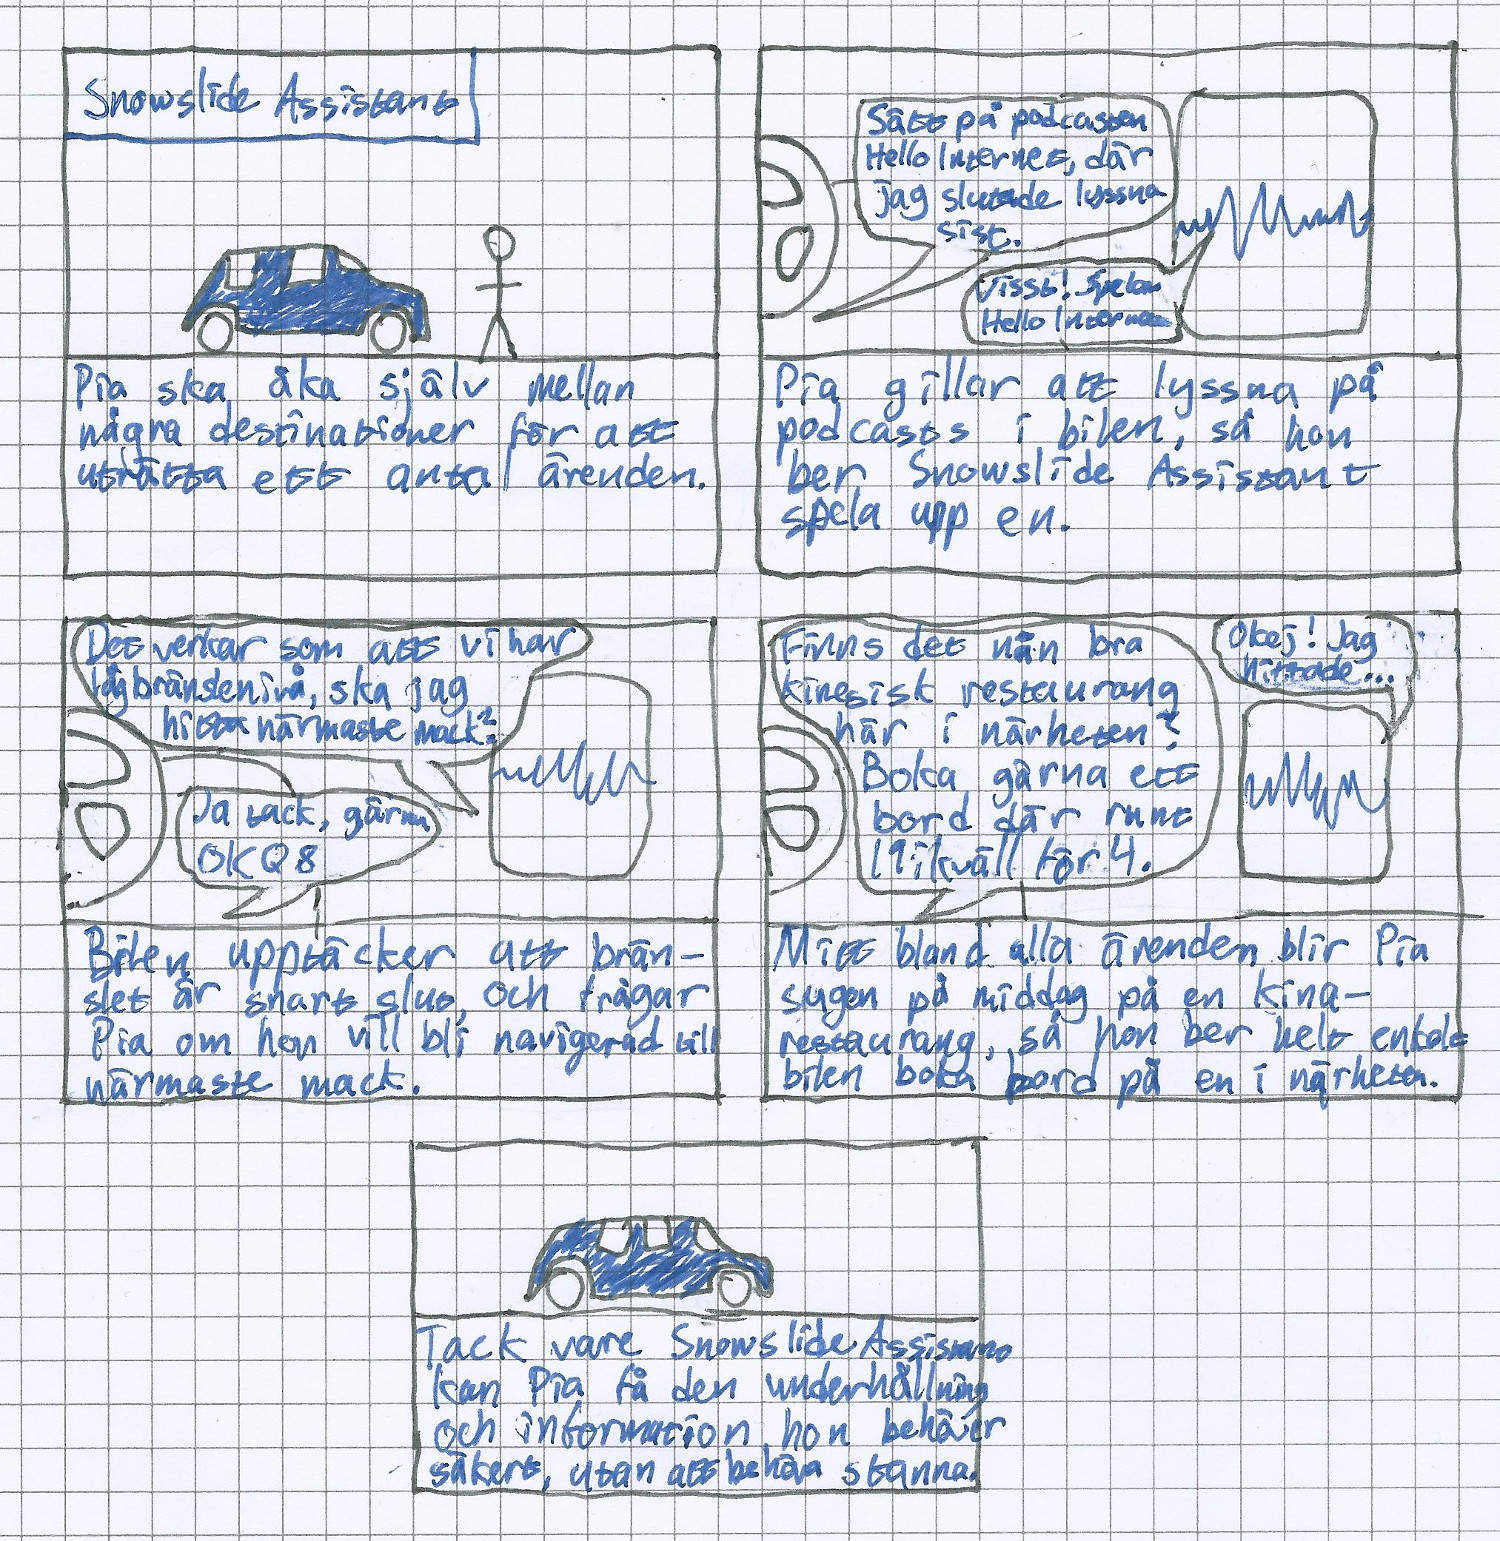
\includegraphics[width=15cm]{images/assistant.jpg}
\end{center}

\newpage
\subsection*{Värderingsmatris}

Kriterierna i värderingsmatrisen inspireras av designmålen för Pia och Tom,
och Snowslide4U väljs som utgångspunkt för värderingsmatrisen:

\renewcommand*{\arraystretch}{1.3}
\begin{longtable}[l]{p{4cm} c c c}
    \textbf{Kriterie} & \textbf{Snowslide4U} & \textbf{Connected} & \textbf{Assistant} \\ \midrule
    Bekvämlighet                                            & 0 & 0  & 0  \\ \midrule
    Lugnar barnen                                           & 0 & +  & -- \\ \midrule
    Begränsar barnens \\ mediekonsumtion                    & 0 & -- & -- \\ \midrule
    Gör att barnen inte ser något olämpligt                 & 0 & -- & -- \\ \midrule
    Sparar tid                                              & 0 & -- & +  \\ \midrule
    Effektiv \\ informationssökning                         & 0 & 0  & +  \\ \midrule
    Imponerar på kunder                                     & 0 & +  & +  \\ \midrule
    Ger Pia förströelse                                     & 0 & +  & 0  \\ \midrule
    Ger information om platser i närheten                   & 0 & +  & +  \\ \midrule
    Håller Tom sysselsatt                                   & 0 & +  & -- \\ \midrule
    Tom kan ta reda på var man kan skaffa koola grejer      & 0 & 0  & -- \\ \midrule
    Tom får kolla på favoritserier                          & 0 & -- & -- \\ \midrule
    Tom kan snabbt gå vidare om han inte hittar något kul   & 0 & 0  & -- \\ \midrule
    Enkelhet att implementera                               & 0 & --  & 0 \\ \midrule
    \textbf{Totalt antal + }      & \textbf{0} & \textbf{5}  & \textbf{4} \\ \midrule
    \textbf{Totalt antal --}      & \textbf{0} & \textbf{5}  & \textbf{7} \\ \midrule
    \textbf{Totalt}      & \textbf{0} & \textbf{0}  & \textbf{-3} \\
\end{longtable}

Värderingsmatrisen visar att Snowslide Connected och Snowslide4U
uppfyller designmålen mer än Snowslide Assistant. Det känns som att Snowslide4U
är mer flexibel och realistisk än Snowslide Connected, vilket är
varför Snowslide4U väljs som koncept att vidareutveckla.

\newpage
\subsection*{Gränssnittsflöden}

Gränssnittsflödena för Snowslide4U delades upp mellan hur det ser ut för passagerare och
förare. Skillnaderna mellan dessa är mest vid uppstart av systemet, då det är
då föraren tilldelar profilerna till sätena.

\textbf{Flöde för passagerare:}
\begin{center}
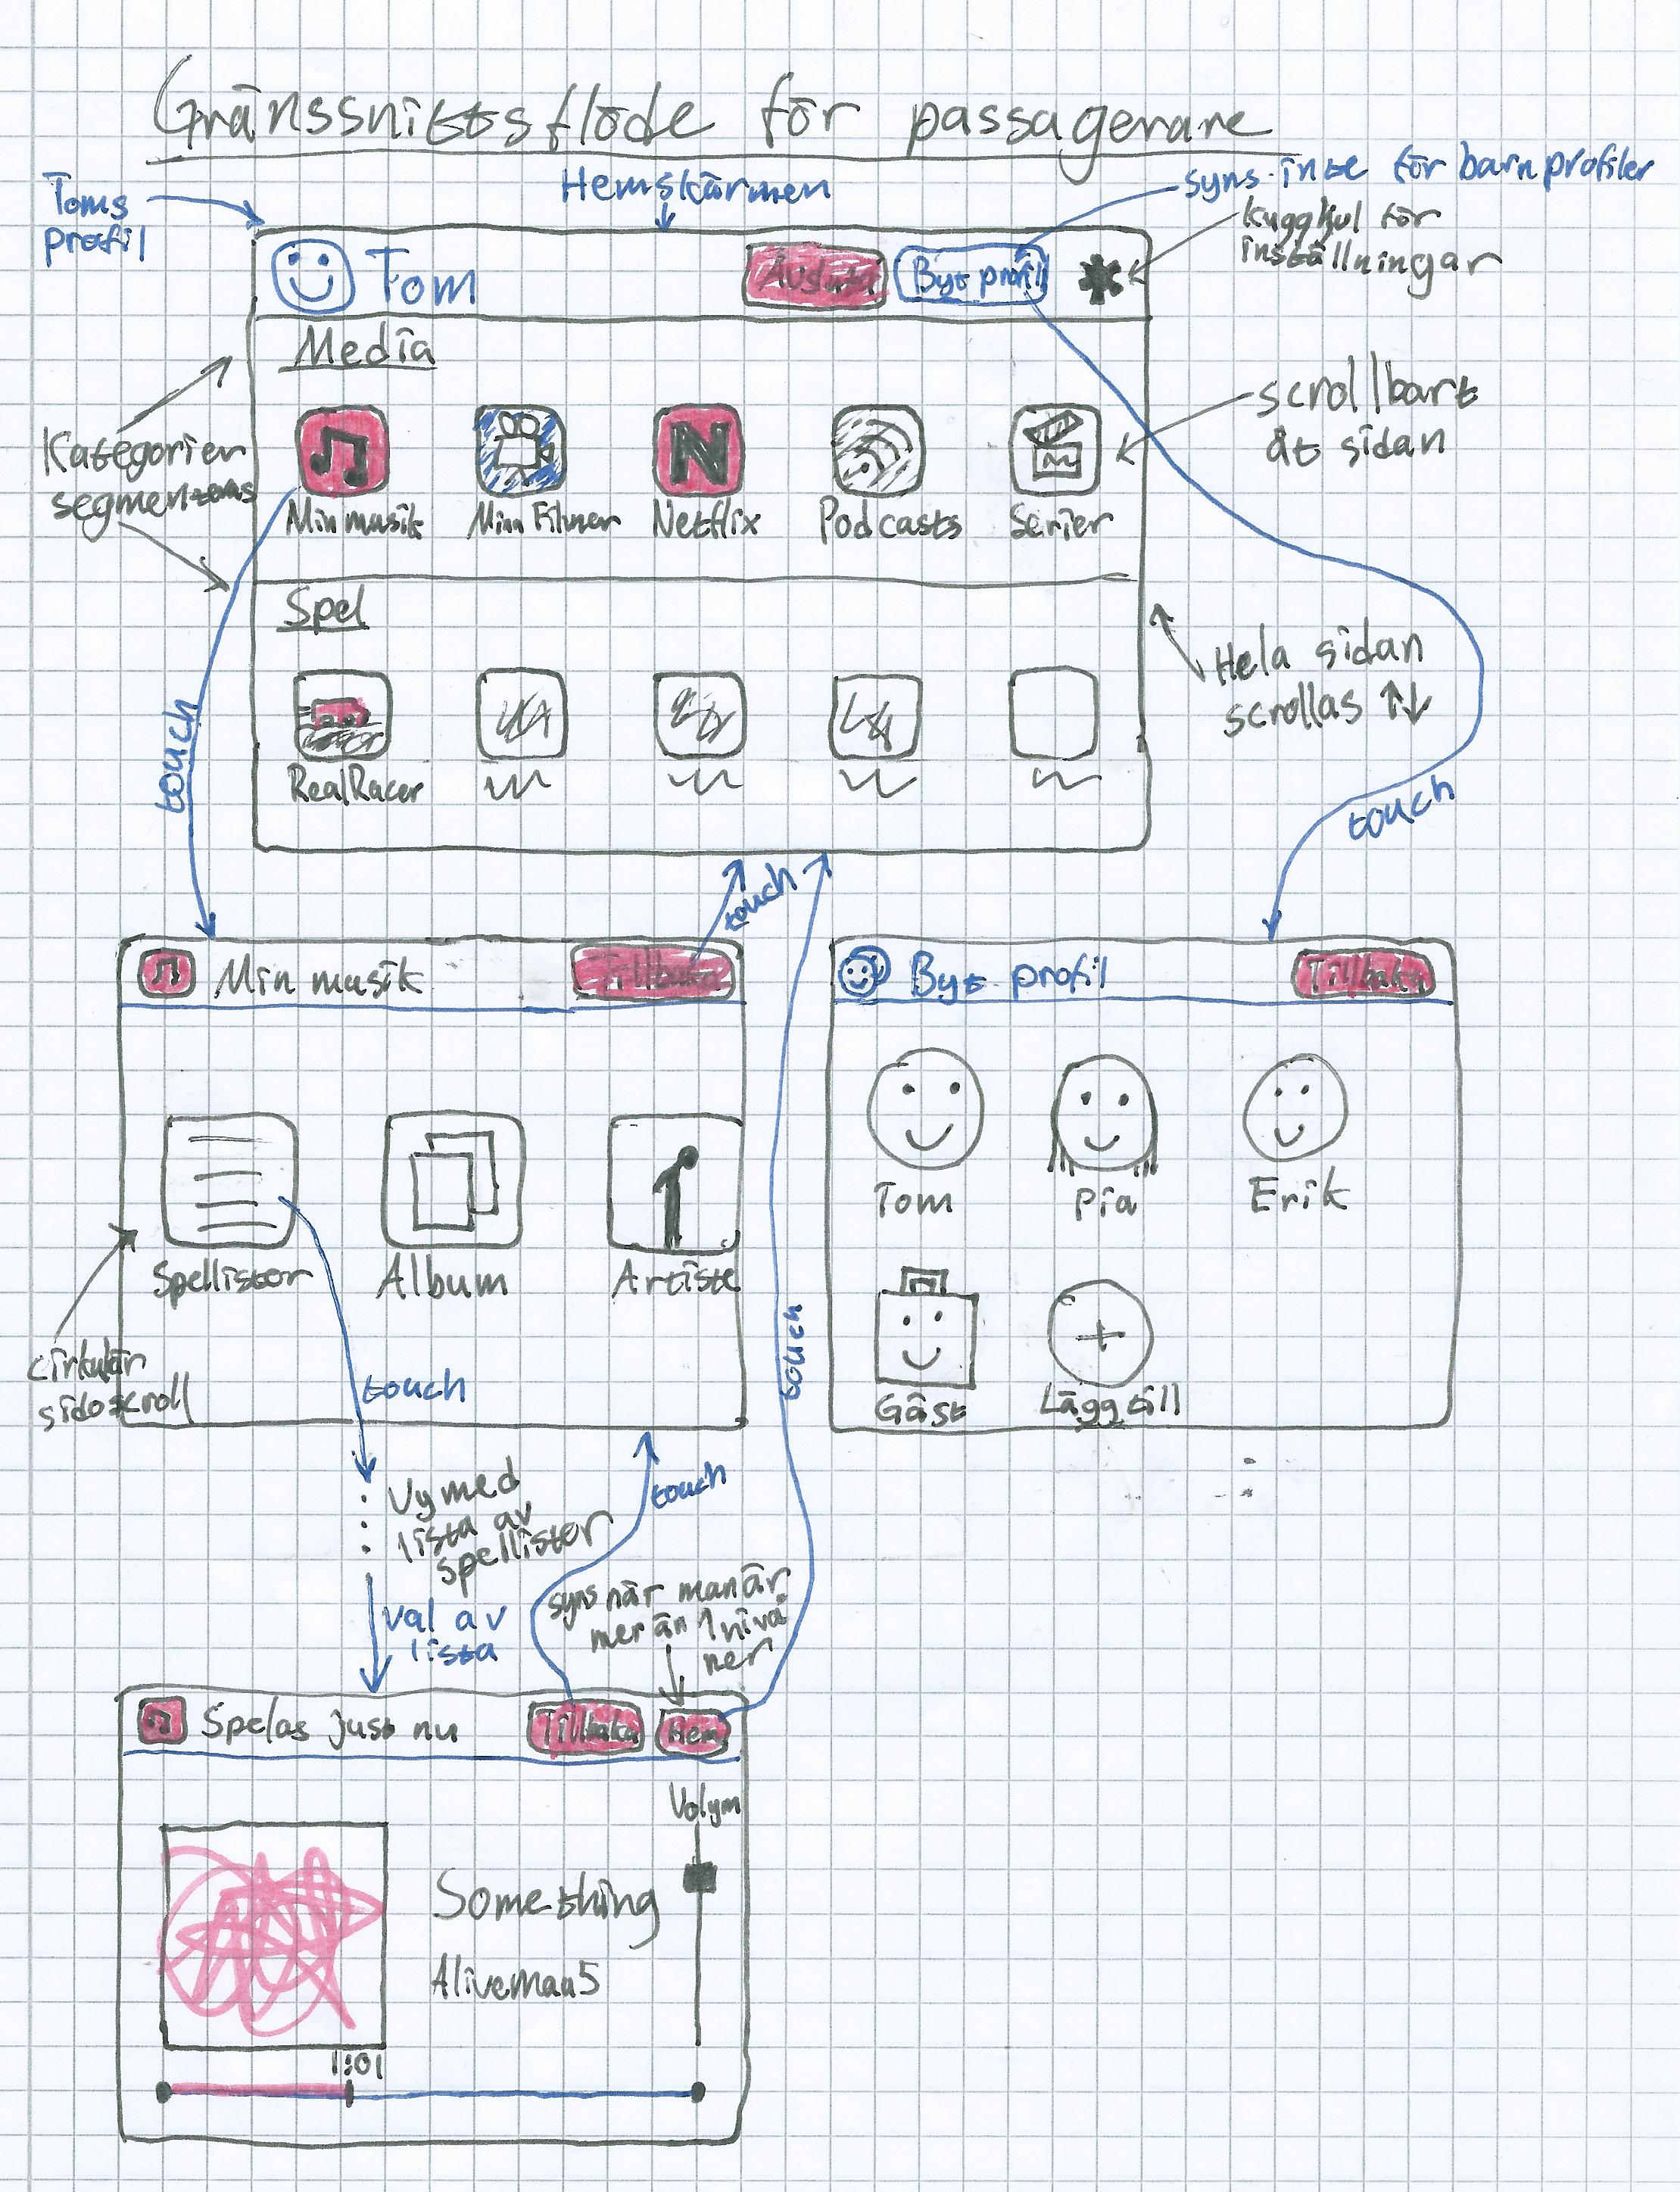
\includegraphics[width=14cm]{images/passflow.jpg}
\end{center}

\newpage
\textbf{Flöde för förare:}
\begin{center}
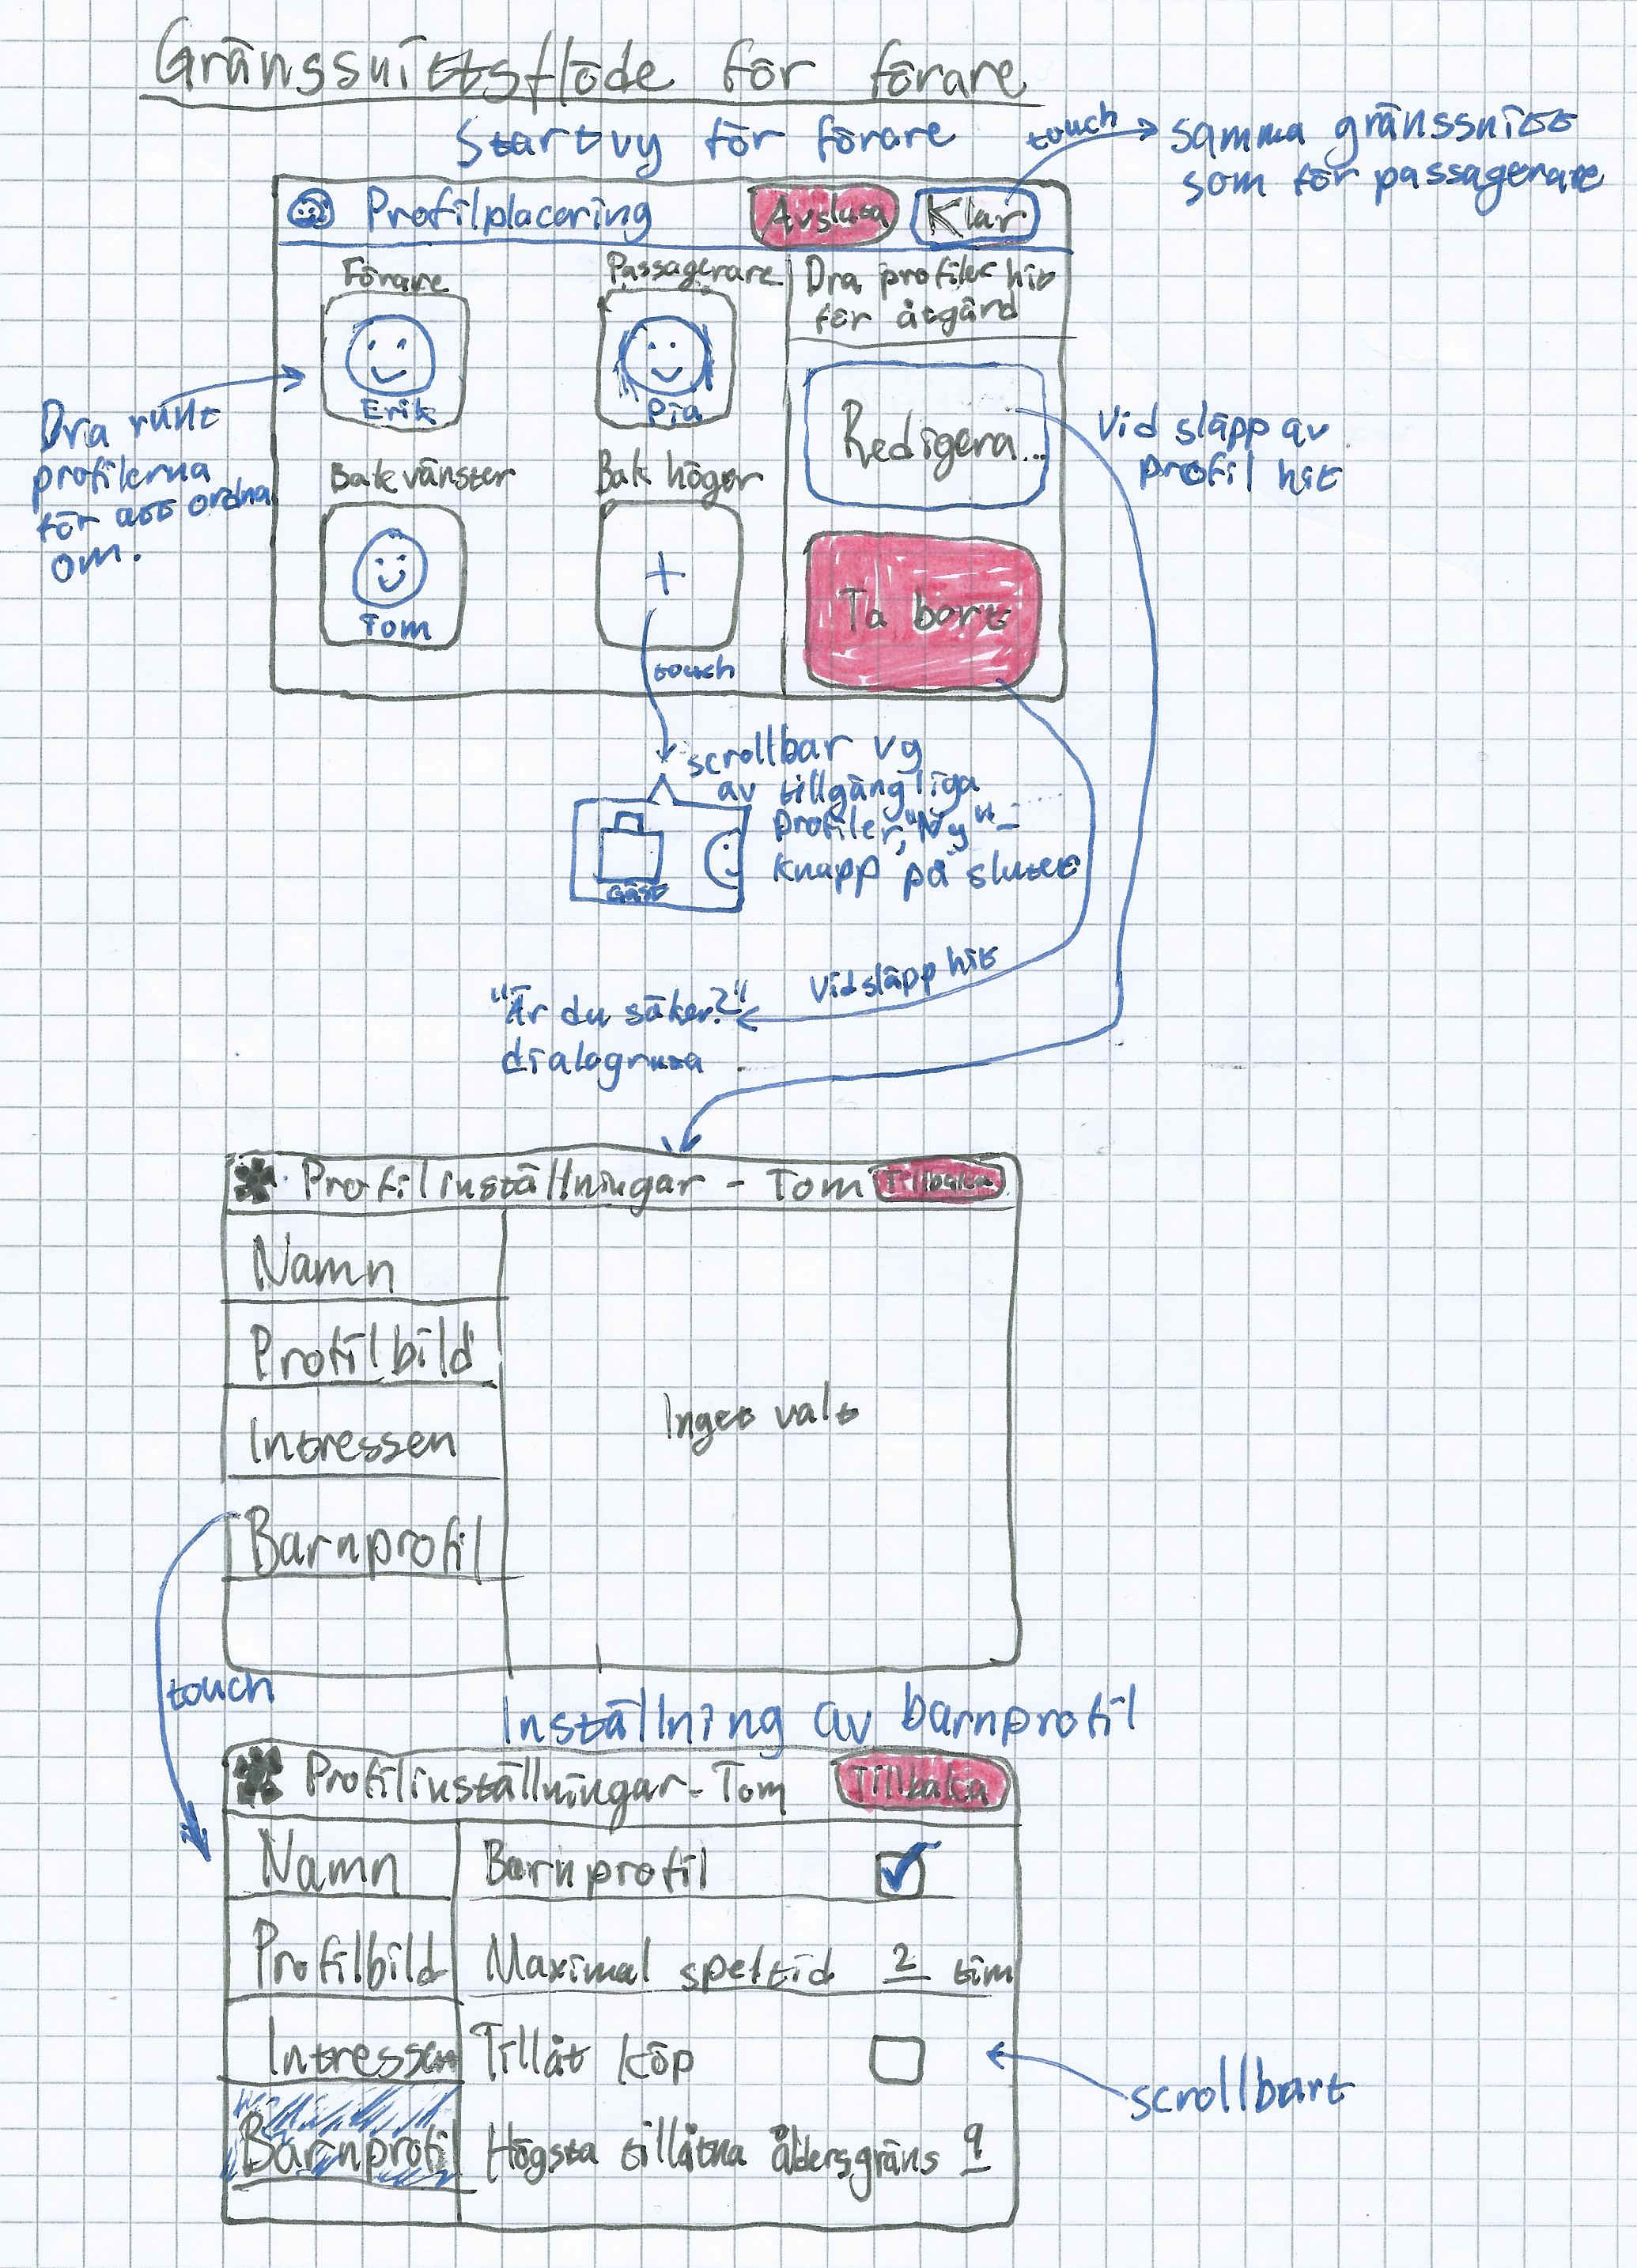
\includegraphics[width=14cm]{images/driverflow.jpg}
\end{center}

\end{document}
